\section{Stern--Gerlach Experiment - 施特恩--格拉赫实验}
This experiment demonstrated that the magnetic moments (a.k.a spins of the electrons) of silver atoms are quantized (that is, it is not a classical degree of freedom).

\subsection{Setup - 实验设置}
\begin{center}
    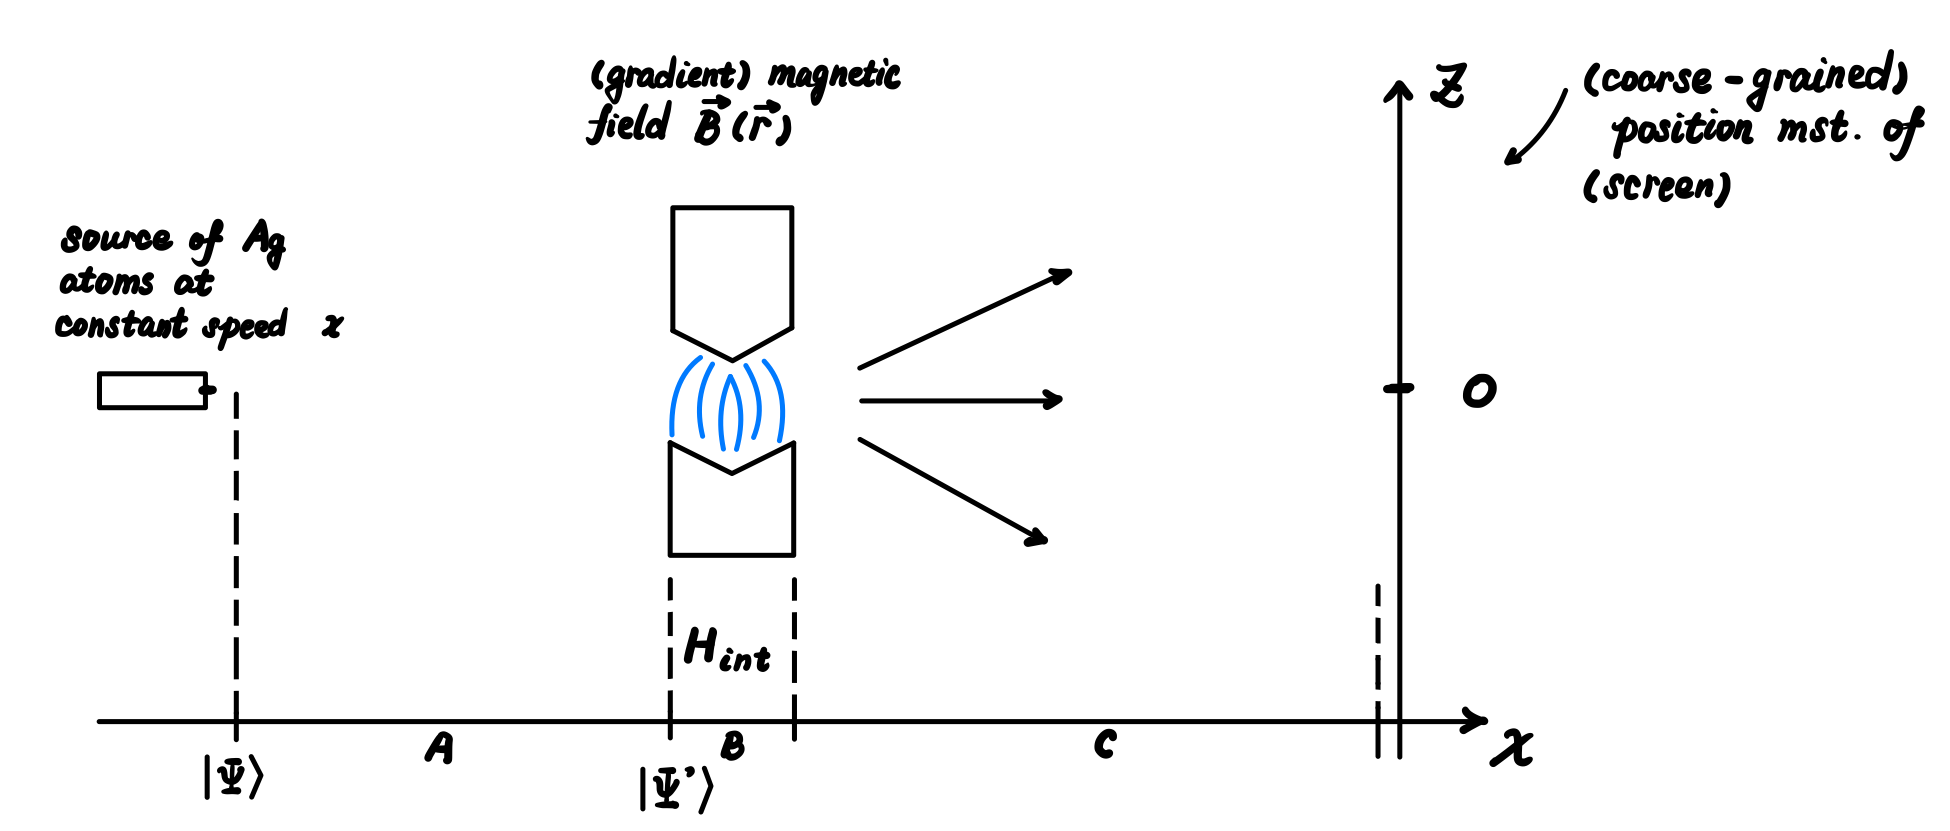
\includegraphics[scale = 0.45]{stern-gerlach-setup.png}
\end{center}
We set up the experiment such that the silver atoms are emitted at a constant speed along the $x$-axis. It will pass through a magnetic field and we observe where it lands on a coarse-grained screen.

\subsection{A First Look - 实验浅尝}
A first look of the experiment assumes that in region $A$ and $C$, the Hamiltonian will be $\hamiltonian = 0$, while in region $B$, the region of interaction, we denote it as $\hamiltonian_{\text{int}}$. We also assume that the speed at emittance remains constant throughout, so the position along the $x$-axis is proportional to time: $x(t) \propto t$. \par
Since we know the Hamiltonian, when viewed as an observable, when measured yields the energy of the total system, so in the interaction region, we have the Hamiltonian to be:
$$\hamiltonian_{\text{int}} = -\vec{\mu} \cdot \vec{B}(\vec{r})$$
where $\vec{\mu}$ is the magnetic moment, $\vec{B}$ is the magnetic field. Here, we approximate the magnetic field is only along the $z$-axis, and the magnetic moment is along the $z$-axis in a Bloch sphere. So the interaction Hamiltonian becomes:
$$\hamiltonian_{\text{int}} = -\mu_z \cdot B_z(\vec{r})$$
If we analyze the experiment classically, the force exerted on the silver atom in the magnetic field should be:
$$\vec{F} = -\nabla\hamiltonian_{\text{int}} = \begin{pmatrix}
    0 \\ 0 \\
    \mu_z \pdv{B_z(\vec{r})}{z}
\end{pmatrix}$$
where the force in $z$-direction should depend on the magnetic moment. Thus, the classical expectation yields that, assuming the magnetic moments in $z$-direction are classical degrees of freedom and they are random from source, the distribution of silver atoms observed on the screen should spread out from the center with the center having the largest density (Gaussian distribution). However, actual observation indicates that the center of the screen has little to none observations but there are two peaks on at positions $+\Delta$ and $-\Delta$. \par
The classical explanation fails to reflect the observation, thus, we need to explain this phenomenon in a quantum model. \par
To start with, we model the quantum system as:
$$\hilbert_{\text{total}} = \hilbert_{\text{magnetic}} \otimes \hilbert_z$$
where $\hilbert_{\text{mag}}$ is spanned by $\{\ket{0}, \ket{1}\}$ ($\ket{0}$ denotes spinning upwards, and $\ket{1}$ denotes spinning downwards), and $\hilbert_z$ is spanned by $\{\ket{z}\}_z$ (a 1D continuous position space). Here, the $x$-direction and $y$-direction are not modelled, as they do not contribute to our analysis. \par
The initial state can thus be modelled as the following:
$$\ketPsi = (\alpha \ket{0} + \beta \ket{1}) \otimes \ketpsi_z$$
where
$$\ketpsi_z = \intR \psi(z)\ket{z} \dd z$$
and $\abs{\psi(z)}^2 \propto -\frac{z^2}{2\sigma^2}$ (a Gaussian random variable). \par
From here on, we wish to understand the evolution of the state. \par
It is trivial to observe that in regions where $\hamiltonian = 0$, the state remains constant as Schr\"odinger's equation demonstrates that the time-derivative of the state is $0$. \par
For the interaction region, classically, we have shown what it is previously. However, in a quantum model, the classical quantities must be promoted to operators/observables:
\begin{align*}
    \hilbert_{\text{int}} &= - (\gamma Z \otimes \id) \cdot (\id \otimes B_z(\vec{r})) \\
    &= -\gamma Z \otimes B_z(\vec{r})
\end{align*}
The corresponding unitary evolution operator will have the following mapping:
$$\opuni: \begin{cases}
    \ket{0} \otimes \ketpsi \mapsto \ket{0} \otimes \mathcal{T}_{+\Delta}\ketpsi \\
    \ket{1} \otimes \ketpsi \mapsto \ket{1} \otimes \mathcal{T}_{-\Delta}\ketpsi
\end{cases}$$
where $\mathcal{T}$ is the translation operator and the subscript is how much the operator translates the state on the $z$-direction. \par
This means, the evolution leads to a magnetic-moment-dependent shift of particle in $\pm \Delta$, where the size of $\Delta$ depends on the strength of $\vec{\mu}, \vec{B}$ and $\nabla\vec{B}$. We assume deflection by $\Delta$ to be visible: $\Delta >> \sigma$. \par
Now, on the final state after evolution, we perform a local position measurement in the $z$-direction. This means, on the magnetic moment space, the operator is $\id_{\text{mag}}$. Since the observation occurs on a coarse-grained screen, we can assume finite precision $\varepsilon > 0$, where the screen can be evenly spaced out by regions of size $\varepsilon$. The projector on the entire state will be:
$$\id \otimes \int_{n\varepsilon}^{(n+1)\varepsilon} \dyad{z} \dd z$$
where $n \in \Z$. Random magnetic moment means random $\alpha, \beta$.

\subsection{Preparation for a Deeper Analysis - 深度分析准备}
With the same setup, we can then consider the 3 dimensional case. Define the Hilbert space to be $\hilbert = \hilbert_x \otimes \hilbert_y \otimes \hilbert_z$. This can be expressed in two ways:
$$\hilbert = \Span{\ket{\vec{r}}}_{\vec{r} \in \R^3} = \Span{\ket{\vec{p}}}_{\vec{p} \in \R^3}$$
where
$$\vec{r} = \begin{pmatrix}
    x \\ y \\ z
\end{pmatrix}, \ket{\vec{r}} = \ket{xyz}; \vec{p} = \begin{pmatrix}
    p_x \\ p_y \\ p_z
\end{pmatrix}, \ket{\vec{p}} = \ket{p_xp_yp_z}$$
The inner product between the two basis state is:
\begin{align*}
    \braket{\vec{r}}{\vec{p}} &= (\bra{x} \otimes \bra{y} \otimes \bra{z})(\ket{p_x} \otimes \ket{p_y} \otimes \ket{p_z}) \\
    &= (2\pi\hbar)^{-\frac{3}{2}} \exp(\frac{\imag \vec{r} \cdot \vec{p}}{\hbar})
\end{align*}
A general state, can also be expressed in two ways:
$$\ketpsi = \int_{\R^3} \psi(\vec{r})\ket{\vec{r}} \dd^3 \vec{r} = \int_{\R^3} \tilde{\psi}(\vec{p})\ket{\vec{p}}\dd^3 \vec{p}$$
The relevant operators/observables are defined as follows:
$$\oppos = \oppos \otimes \id_y \otimes \id_z, \opmtm_x = \opmtm_x \otimes \id_y \otimes \id_z, \dots$$
where the operators act on the wavefunctions in these ways:
\begin{align*}
    \oppos&: \begin{cases}
        \psi(\vec{r}) \mapsto x\psi(\vec{r}) \\
        \tilde{\psi}(\vec{p}) \mapsto \imag \hbar \pdv{p_x}\tilde{\psi}(\vec{p})
    \end{cases} \\
    \opmtm_y&: \begin{cases}
        \psi(\vec{r}) \mapsto -\imag \hbar \pdv{y}\psi(\vec{r}) \\
        \tilde{\psi}(\vec{p}) \mapsto p_y\tilde{\psi}(\vec{p})
    \end{cases}
\end{align*}
Consequently, we consider two vectors of operators being:
$$\opmtm = \begin{pmatrix}
    \opmtm_x \\ \opmtm_y \opmtm_z
\end{pmatrix}, \hat{R} = \begin{pmatrix}
    \oppos \\ \hat{Y} \\ \hat{Z}
\end{pmatrix}$$
where $\hat{R}^2 = \oppos^2 + \hat{Y}^2 + \hat{Z}^2$, and when $\opmtm^2$ is applied to $\psi(\vec{r})$, we have:
$$\opmtm^2: \psi(\vec{r}) \mapsto -\hbar^2 \nabla^2 \psi(\vec{r})$$
The key commutators are:
$$[\oppos, \opmtm_x] = [\hat{Y}, \opmtm_y] = [\hat{Z}, \opmtm_z] = \imag \hbar \id_x \otimes \id_y \otimes \id_z$$

\subsection{Deeper Analysis - 深度分析}
We model the quantum system with $\hilbert = \hilbert_s \otimes \hilbert_x \otimes \hilbert_z$, where $\hilbert_s = \Span{\ket{0}, \ket{1}}$ and the other two are the corresponding position spaces. The Hamiltonian will be in two parts:
$$\hamiltonian_{sxz} = \hamiltonian_0 + \hamiltonian_{\text{interaction}}$$
where $\hamiltonian_0 = \frac{1}{2\mu}(\opmtm_x^2 + \opmtm_z^2)$, the interaction Hamiltonian should model the magnetic field:
$$\hamiltonian_{\text{int}} = \gamma \cdot Z \otimes \proj{x}^{[0, \delta]} \otimes \hat{Z}$$
This is essentially derived from $\hamiltonian_{\text{int}} = -\vec{\mu} \cdot \vec{B}$. For spin-$\frac{1}{2}$ atoms:
$$\vec{\mu} \propto \begin{pmatrix}
    X \otimes \id \otimes \id \\
    Y \otimes \id \otimes \id \\
    Z \otimes \id \otimes \id
\end{pmatrix}$$
and the magnetic field is a gradient in spatial $z$-direction and only non-zero for $x \in [0, \delta]$, so:
$$\vec{B}(\hat{R}) \propto \begin{pmatrix}
    0 \\ 0 \\
    \id \otimes \proj{x}^{[0, \delta]} \otimes \hat{Z}
\end{pmatrix}$$
Thus, when multiplied together, we have $\hamiltonian_{\text{int}}$, where $\gamma$ is dependent on the magnetic field strength, coupling constant of the spin to the magnetic field. \par
With the Hilbert space set up, we can have the initial state to be:
$$\ketPsi_{sxz} = (\alpha \ket{0} + \beta \ket{1}) \otimes \ket{\psi_0}_{xz}$$
with the initial position wavefunction to be:
$$\psi_0(x, z) = (\frac{1}{\sqrt[4]{2\pi\sigma^2}})^2\exp(-\frac{(x-x_0)^2}{4\sigma^2}-\frac{(z-z_0)^2}{4\sigma^2}+\imag k x)$$
This represents a Gaussian wavepacket in the $x,z$ directions and an initial momentum in $x$ direction travelling from left to right.
\begin{center}
    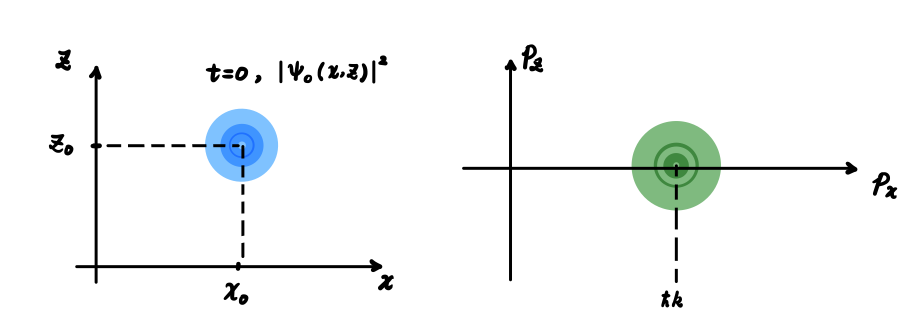
\includegraphics[scale = 1]{stern-gerlach-initial.png}
\end{center}
The time evolution is hard to solve because the unitary propagator is:
$$\opuni(t) = \exp(-\frac{\imag t}{\hbar}(\hamiltonian_0 + \hamiltonian_{\text{int}}))$$
where $\exp(A+B) \ne \exp(A) + \exp(B)$ if $[A, B] \ne 0$. \par
We can first conduct a semi-classical analysis separately per region. For regions $A, C$, the \impt{support} (the part of function that is only larger than $\varepsilon$) of the position wavefunction
$$\text{supp}_\varepsilon(\psi_{xz}) \cap [0, \delta] \approx \varnothing$$
We then can approximate:
$$\hamiltonian_{\text{int}} \ketPsi \approx 0 \to \opuni_{AC}(t) \approx \exp(-\frac{\imag t}{\hbar}\hamiltonian_0) = \id \otimes \exp(-\frac{\imag t}{2\mu\hbar}\opmtm_x^2) \otimes \exp(-\frac{\imag t}{2\mu\hbar}\opmtm_z^2)$$
With the Ehrenfest Relations in \hyperref[subsec:ehrenfest]{\textcolor{cyan}{Section 5.2}}, we have two sets of relationship:
\begin{align*}
    \expval{\oppos}_t &= \expval{\oppos}_0 + t \cdot \frac{\expval{\opmtm_x}_0}{\mu} = x_0 + t \cdot \frac{\hbar k}{\mu} \\
    \expval{\opmtm_x}_t &= \expval{\opmtm_x}_0= \hbar k \\
    (\Delta \oppos)_t^2 &= \sigma^2 + \frac{\hbar^2}{4\sigma^2\mu^2} \cdot t^2 \\
    (\Delta \opmtm_x)_t^2 &= \frac{\hbar^2}{4\sigma^2} \\
    \expval{\hat{Z}}_t &= \expval{\hat{Z}}_0 + t \cdot \frac{\expval{\opmtm_z}_0}{\mu} = z_0 \\
    \expval{\opmtm_z}_t &= \expval{\opmtm_z}_0= 0 \\
    (\Delta \hat{Z})_t^2 &= \sigma^2 + \frac{\hbar^2}{4\sigma^2\mu^2} \cdot t^2 \\
    (\Delta \opmtm_z)_t^2 &= \frac{\hbar^2}{4\sigma^2}
\end{align*}
\begin{center}
    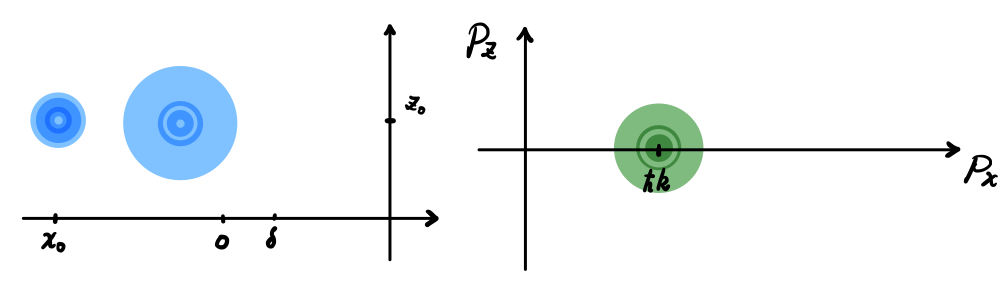
\includegraphics[scale = 0.8]{stern-gerlach-nonint.png}
\end{center}
For region $B$, we can assume a strong magnetic field and strong coupling to approximate $\hamiltonian$ to be $\hamiltonian_{\text{int}}$ only.
\begin{lemma}
    Consider an operator $A$ and a projector $\Pi$, we have
    $$e^{A \otimes \Pi} = e^A \otimes \Pi + \id \otimes (\id - \Pi)$$
\end{lemma}
So the unitary propagator is:
$$\opuni_B(t)_{szx} \approx \exp(-\frac{\imag t}{\hbar} \hamiltonian_{\text{int}}) = \exp(-\frac{\imag t \gamma}{\hbar}(Z \otimes \hat{Z})) \otimes \proj{x}^{[0, \delta]} + (\id \otimes \id) \otimes (\id - \proj{x}^{[0, \delta]})$$
We specifically need to investigate how $\exp(-\frac{\imag t \gamma}{\hbar}(Z \otimes \hat{Z}))$ acts on $\hilbert_s \otimes \hilbert_z$. Consider an arbitrary state $\ketPhi_{sz} = (\alpha \ket{0} + \beta \ket{1}) \otimes \ketphi_z$, this operator yields:
\begin{align*}
    \exp(-\frac{\imag t \gamma}{\hbar}(Z \otimes \hat{Z})) \ketPhi_{sz} &= \alpha\exp(-\frac{\imag t \gamma}{\hbar}(Z \otimes \hat{Z})) \ket{0}\ket{\phi} \\
    &+ \beta\exp(-\frac{\imag t \gamma}{\hbar}(Z \otimes \hat{Z})) \ket{1}\ket{\phi}
\end{align*}
Through mathematical manipulation (skipped here), we finally have:
$$\alpha \ket{0} \otimes \exp(-\frac{\imag t \gamma}{\hbar}\hat{Z})\ketphi_z + \beta \ket{1} \otimes \exp(+\frac{\imag t \gamma}{\hbar}\hat{Z})\ketphi_z$$
We then investigate the behaviour of: $\exp(\pm\frac{\imag t \gamma}{\hbar}\hat{Z})$.
\begin{align*}
    \psi(z) &\mapsto \exp(\pm \frac{\imag t \gamma}{\hbar}z)\phi(z) \\
    \tilde{\psi}(p_z) &\mapsto \tilde{\psi}(p \pm t\gamma)
\end{align*}
where the second relation is conducted through Fourier transform.
\begin{center}
    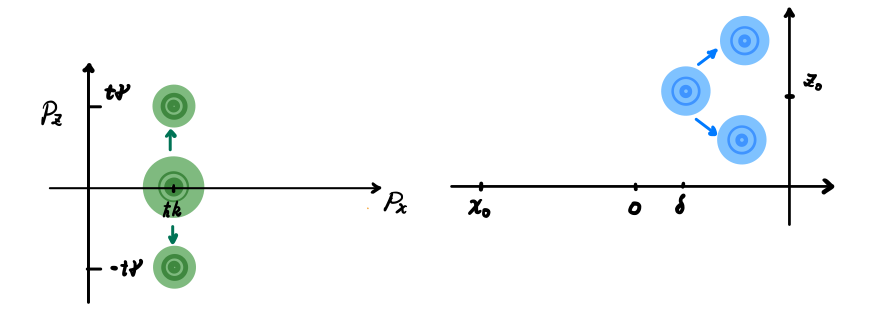
\includegraphics[scale = 1]{stern-gerlach-int.png}
\end{center}
When the wavepacket reached the screen, the state will be:
$$\ket{\Psi'}_{sxz} = \alpha\ket{0}_s \otimes \ket{\psi_+}_{xz} + \beta\ket{1}_s \otimes \ket{\psi_-}_{xz}$$
Finally, when we conduct a position measurement with the projectors to be: $\{\proj{n\varepsilon}\}_{n \in \Z - \{0\}}$, where each projector is:
$$\proj{n\varepsilon} = \id \otimes \id \otimes \int_{n\varepsilon}^{(n+1)\varepsilon} \dyad{z} \dd z$$
The probability is thus:
\begin{align*}
    \Prob{n} &= \expval{\proj{n\varepsilon}}{\Psi'} \\
    &= \abs{\alpha}^2 \cdot \intR \int_{n\varepsilon}^{(n+1)\varepsilon} \abs{\psi_+(x, z)}^2 \dd z \dd x \\
    &+ \abs{\beta}^2 \cdot \intR \int_{n\varepsilon}^{(n+1)\varepsilon} \abs{\psi_-(x, z)}^2 \dd z \dd x
\end{align*}
The post-measurment state is thus:
$$\frac{\proj{n\varepsilon}\ket{\Psi'}_{sxz}}{\sqrt{\Prob{n}}}$$
\begin{center}
    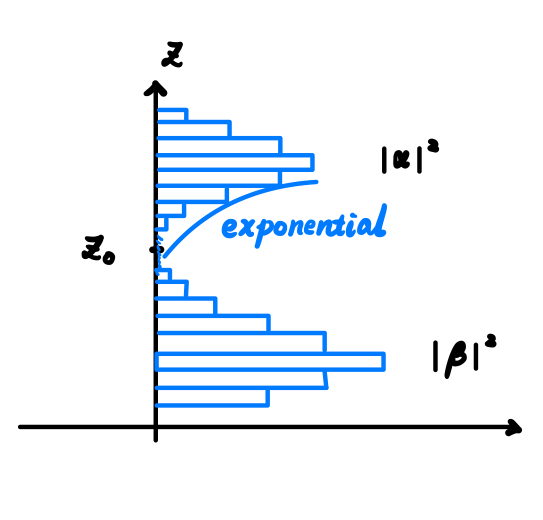
\includegraphics[scale = 0.5]{stern-gerlach-outcome.png}
\end{center}

\newpage